\documentclass[addpoints]{exam}
\usepackage{amsmath}
\usepackage{amssymb}
\usepackage{listings}
\usepackage{pxfonts}
\usepackage{xcolor}
\usepackage{multirow}
\usepackage{array}
\usepackage{tikz}
\usepackage{forest}
\lstset{language=Python,
	basicstyle=\ttfamily,
	keywordstyle=\bfseries,
	showstringspaces=false,
	morekeywords={if, else, then, print, end, for, do, while,output},
	tabsize=4,
	mathescape=true,
	moredelim=**[is][\color{red}]{@}{@},
}
    \setlength{\extrarowheight}{2pt}
\pagestyle{headandfoot}
\firstpageheadrule
\runningheadrule
\firstpageheader{Algorithmic Game Theory}{}{mbkb74}
\runningheader{Algorithmic Game Theory}{Individual Component}{mbkb74}
\firstpagefooter{}{}{}
\runningfooter{}{}{}
\renewcommand{\solutiontitle}{\noindent\textbf{Answer:}\par\noindent}


\printanswers
\usepackage{graphicx}
\marksnotpoints
\bracketedpoints
\pointsdroppedatright
\pointsinrightmargin
\begin{document}
\begin{center}
    \LARGE{Algorithmic Game Theory Summative Assignment -- Individual Component}\\[0.1cm]
\end{center}

\begin{questions}

    \question 	      Consider the following instance of the load balancing game where the number of tasks is equal to the number of machines, and in particular we have:
    \begin{itemize}
        \item $m$ identical machines $M_1, M_2, \dots, M_m$ (all of speed 1),
        \item $m$ identical tasks $w_1 = w_2 = \dots = w_m = 1$.
    \end{itemize}
    Consider also the mixed strategy profile $A$ where each of the tasks is assigned to all machines equiprobably (i.e. with probability $1/m$).
    \begin{parts}
        \part[3]Calculate the ratio $cost(A)/cost(OPT)$ in the special case where $m=2$.
        \begin{solution}[2in]
            \begin{itemize}
                \item There are $2^2=4$ possible assignments of 2 tasks to 2 machines
                \item In two of these both tasks are assigned to 1 machine (time 2)
                \item In the other two one task is assigned to each machine (time 1)
                \item The Cost of A is therefore $1/4(2+2+1+1)=1.5$
                \item However the optimal cost is where one is assigned to each machine $1$
                \item The ratio is therefore 1.5
            \end{itemize}
        \end{solution}
        \part[3]Calculate the ratio $cost(A)/cost(OPT)$ in the special case where $m=3$.
        \begin{solution}[2in]
            For 3 machines and 3 tasks there are $3^3=27$ possible assignments, of which
            \begin{itemize}
                \item 6 take time 1
                \item 18 take time 2
                \item 3 take time 3
            \end{itemize}
            The cost of A is therefore
            $$
                \dfrac{1}{27}(3\times 3 + 1\times 6 + 2\times 18)=\dfrac{17}{9}
            $$
            The optimal cost is still 1, so the ratio is $\dfrac{17}{9}$
        \end{solution}
        \part[5]Discuss what this ratio is for arbitrary $m$. What does this imply about the Price of Anarchy on identical machines for mixed Nash equilibria?
        \begin{solution}[2in]
            To put a simple upper bound on the ratio, if you assume that instead of the distribution it currently takes, that instead all the possible assignments were the worst case of taking $m$.

            This would make the cost of A
            $$
                \dfrac{1}{n^n}(n\times n^n)
            $$

            Which would be simply $n$
        \end{solution}
    \end{parts}
    \droptotalpoints

    \question 	      	      We consider a second-price sealed-bid auction where there are $n$ bidders who bid as follows:
    \begin{itemize}
        \item Bidders 1 up to $n-1$ bid either 1 dollar or $r > 1$ dollars equiprobably and
              independently of the rest.
        \item Bidder $n$ bids $h$ dollars, where $h > r$.
    \end{itemize}
    The seller's expected revenue $R$ is the expectation of the second highest value.
    \begin{parts}
        \part[1]What is the value that $R$ is approaching when $n$ is very large?
        \begin{solution}[2in]
            $$
                r
            $$
        \end{solution}
        \part[9]Justify your answer by taking the limit.
        \begin{solution}[2in]
        \end{solution}
    \end{parts}
    \droptotalpoints

    \question 	      Mary and Alice are buying items for Sunday lunch. Mary buys either chicken $(C)$ or beef $(B)$ for the main course and Alice buys either juice $(J)$
    or wine $(W)$. Both people prefer wine with beef and juice with chicken. The opposite alternatives are equally displeasing.
    However, Mary prefers beef over chicken, while Alice prefers chicken over beef.

    We assume that Mary buys first and then tells Alice what she bought,
    so when Alice makes her decision, she knows if the main course is beef or chicken.
    \begin{parts}
        \part[2]Express the above preferences as payoffs by using numbers\\(e.g.
        $u_M(B,W) = 2$, $u_A(B,W) = \ldots$  etc.)
        \begin{solution}[2in]
            \begin{itemize}
                \item $u_M(B,W)=2$
                \item $u_A(B,W)=1$
                \item $u_M(C,W)=0$
                \item $u_A(C,W)=0$
                \item $u_M(C,J)=1$
                \item $u_A(C,J)=2$
                \item $u_M(B,J)=0$
                \item $u_A(B,J)=0$
            \end{itemize}
        \end{solution}
        \part[4]Write down a bimatrix game with Mary as the row player
        and Alice as the column player, using your chosen payoffs.
        \begin{solution}[2in]


            \begin{tabular}{cc|c|c|}
                                     & \multicolumn{1}{c}{} & \multicolumn{2}{c}{Mary}                               \\
                                     & \multicolumn{1}{c}{} & \multicolumn{1}{c}{Chicken} & \multicolumn{1}{c}{Beef} \\\cline{3-4}
                \multirow{2}*{Alice} & Juice                & $(1,2)$                     & $(0,0)$                  \\\cline{3-4}
                                     & Wine                 & $(0,0)$                     & $(2,1)$                  \\\cline{3-4}
            \end{tabular}

        \end{solution}
        \part[4]Write down a game tree representing this game as an extended game.
        \begin{solution}[2in]
            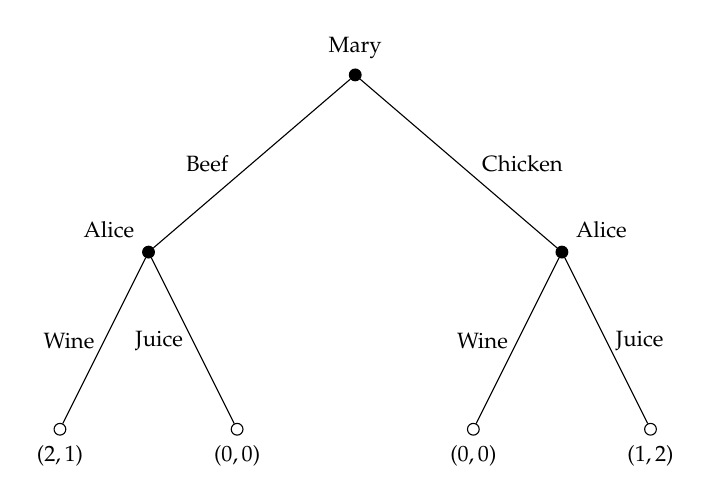
\begin{tikzpicture}[scale=1.5,font=\footnotesize]
                \tikzstyle{solid node}=[circle,draw,inner sep=1.5,fill=black]
                \tikzstyle{hollow node}=[circle,draw,inner sep=1.5]
                \tikzstyle{level 1}=[level distance=15mm,sibling distance=3.5cm]
                \tikzstyle{level 2}=[level distance=15mm,sibling distance=1.5cm]
                \tikzstyle{level 3}=[level distance=15mm,sibling distance=1cm]
                \node(0)[solid node,label=above:{Mary}]{}
                child{node[solid node,label=above left:{Alice}]{}
                child{node[hollow node,label=below:{$(2,1)$}]{} edge from parent node[left]{Wine}}
                child{node[hollow node,label=below:{$(0,0)$}]{} edge from parent node[left]{Juice}}
                edge from parent node[left,xshift=-5]{Beef}
                }
                child{node[solid node,label=above right:{Alice}]{}
                child{node[hollow node,label=below:{$(0,0)$}]{} edge from parent node[left]{Wine}}
                child{node[hollow node,label=below:{$(1,2)$}]{} edge from parent node[right]{Juice}}
                edge from parent node[right,xshift=5]{Chicken}
                };
            \end{tikzpicture}
        \end{solution}
        \part[5]Find a solution for the extended game using backward induction.\\Describe your steps.
        \begin{solution}[2in]
            \begin{itemize}
                \item Mary can reason that if they choose beef then Alice will choose wine, because doing so is better than having Beef with Juice
                \item Given that Mary will respond in this way, Mary is better off choosing Beef
            \end{itemize}
        \end{solution}
    \end{parts}
    \droptotalpoints
    \newpage
    \question 	      	      We consider a (matching) market of $k$ sellers and $k$ buyers, where $k$ is an integer, $k>0$.
    Each seller sells an item and the prices of the items are initially all zero. Buyer $i$ has valuation $k-i+1$ for the first item and valuation $0$ for every other item, as shown in the following diagram.

    \vspace*{0.5cm}
    \begin{tabular}{c r c c c}
        Buyers   & \multicolumn{4}{c}{Valuations (for items $1$ to $k$)}                          \\
        \hline
        $x_1$    & $k,$                                                  & $0,$ & $\ldots,$ & $0$ \\
        $x_2$    & $k-1,$                                                & $0,$ & $\ldots,$ & $0$ \\
        $\vdots$ &                                                       &      & $\vdots$        \\
        $x_k$    & $1,$                                                  & $0,$ & $\ldots,$ & $0$ \\
    \end{tabular}

    \noindent The sellers find the market-clearing prices using the procedure discussed in the lectures.
    \begin{parts}
        \part[3]What are the prices of the sellers' items ($1^{st}$ item, $2^{nd}$ item, \ldots, $k^{th}$ item) when the market clears? Which buyer gets the $1^{st}$ item and at what price?
        \begin{solution}[2in]
            The first item has a price of $k-1$ and the remaining items all have a price of 0. The first buyer gets the 1st item at price $k-1$
        \end{solution}
        \part[6]Justify your answers to (a).
        \begin{solution}[2in]
            Initially set the prices for all the items to 0. In this case all the buyers want to buy item 1 as they have valuation $\geqslant 1$ for that item and 0 for the others. By raising the price of item 1 by 1 the kth buyer now has k preferred sellers, as they get payoff of 0 for item 1 as it has price 1 and they value it at 1 and they get payoff of 0 for the rest of the items as they have price 0 and they value them at 0.

            By continuing to raise the price of item 1, each buyer from $k$ to $3$ no longer becomes interested in the first item, and is now equally interested in the rest of the items. At a price of $k-1$ buyers 1 and 2 are both interested in item 1, but buyer 2 is also interested in the rest of the items, giving a perfect matching where every buyer buys the item associated with their number. (Along with lots of other perfect matchings as buyers $2$ through to $k$ can buy any of the items, as long as no two buy the same)
        \end{solution}
        \part[3]Which kind of auction does the construction of market-clearing prices procedure implement in this case?
        \begin{solution}[2in]
            An English auction as the price increases until buyers are no longer interested as the price has exceeded their valuation
        \end{solution}
    \end{parts}
    \droptotalpoints


\end{questions}





\end{document}




